\documentclass[t,10pt,compress=false,usepdftitle=false]{beamer}

\usetheme[compress]{LMU}
\setbeamercovered{dynamic} % shows items in white grey before active

%no navigational bars:
\setbeamertemplate{navigation symbols}{}

\usepackage[utf8x]{inputenc}
\usepackage[ngerman]{babel}
\usepackage{listings}   % syntax highlighting
\usepackage{courier}
\usepackage{xcolor}
\usepackage{verbatim}

% http://stackoverflow.com/questions/1662037/how-to-write-programming-code-containing-the-character-in-latex
\makeatletter
\let \@sverbatim \@verbatim
\def \@verbatim {\@sverbatim \verbatimplus}
{\catcode`'=13 \gdef \verbatimplus{\catcode`'=13 \chardef '=13 }} 
\makeatother


%\usepackage{amsmath}
%\usepackage{amssymb}

% -----------------------------------------------------------------------------
%
%\newtheorem{definition}{Definition}
\newcommand{\foot}[1]{_{\mbox{\footnotesize #1}}}
\newcommand{\head}[1]{^{\mbox{\footnotesize #1}}}
%
%
\newcommand{\ones}{\mathbb{I}}
\newcommand{\nat}{\mathbb{N}}
\newcommand{\real}{\mathbb{R}}
\newcommand{\ganz}{\mathbb{Z}}
%
%
\newcommand{\RRE}{\mbox{RRE}}
\newcommand{\nnz}[1]{\mbox{nnz}(#1)}
\newlength{\Hoehe}
\renewcommand{\vec}[1]{#1}
\newlength{\GLaenge}
\setlength{\GLaenge}{3.5cm}
%
%
\definecolor{MyGrey}{gray}{0.45}
\def\bstheta{\boldsymbol{\theta}}
\def\bsalpha{\boldsymbol{\alpha}}
\def\bsk{\boldsymbol{k}}
\def\bsx{\boldsymbol{x}}
\def\bsh{\boldsymbol{h}}
%
% Centred minipage environment
%
\newenvironment{cmpage}[1]{
\begin{center}
\begin{minipage}{#1\textwidth}}%
{\end{minipage}\end{center}}
%
%
\newcommand{\POS}{\color{blue}\item [\boldmath{$+$}]}
\newcommand{\NEG}{\color{red}\item [{\boldmath$-$}]}
\newcommand{\NTR}{\color{black}\item [$\circ$]}
\newcommand{\f}[1]{\mathfrak{#1}}
\newcommand{\old}{^{\mbox{\small \color{blue} old}}}
\newcommand{\new}{^{\mbox{\small \color{red} new}}}
\newcommand{\diag}[1]{\mbox{diag}\left(#1\right)}
%
%
\newcommand{\myBlank}{\textvisiblespace}
\newcommand{\noSpace}{\makebox[0pt]{\quad}}
%
% Old style colour commands
%
\newcommand{\CB}{\color{blue}}
\newcommand{\CR}{\color{red}}
\newcommand{\CG}{\color{green}}
\newcommand{\CC}{\color{cyan}}
%
\definecolor{myWhite}{rgb}{1.00,1.00,1.00}  % real white
\definecolor{myGrey}{rgb}{0.78,0.83,0.94}   % 'light grey blue'
\definecolor{myYellow}{rgb}{1.00,1.00,0.00} % yellow
\definecolor{myOrange}{rgb}{1.00,0.65,0.00} % orange
\definecolor{myCyan}{rgb}{0.00,1.00,1.00}   % cyan
%
% Some abbrevs for setting brief code parts
%
\newcommand{\ttA}{\mbox{\texttt{A}}}
\newcommand{\ttB}{\mbox{\texttt{B}}}
\newcommand{\ttC}{\mbox{\texttt{C}}}
\newcommand{\ttD}{\mbox{\texttt{D}}}
\newcommand{\code}[1]{\mbox{\texttt{#1}}}
\newcommand{\ccode}[1]{\cemphd{\texttt{#1}}}
%
% Commands for slides taken from 'Insides'
%
\newcommand{\rst}{\textcolor{emphcolora}{\ast}}
\newcommand{\bst}{\textcolor{emphcolorb}{\ast}}
%
%
%
\definecolor{textcolor} {rgb}{0,0,0}
\definecolor{decocolor} {rgb}{0,0,0}
\definecolor{emphcolora}{rgb}{1,0,0}              % pure red
\definecolor{emphcolorb}{rgb}{0,0,1}              % pure blue
\definecolor{emphcolorc}{cmyk}{0,1,0,0}           % pure magenta
%\definecolor{emphcolord}{cmyk}{0.64,0,0.95,0.20} % sort of green
\definecolor{emphcolord}{rgb}{0,0.4,0.12}         % same as lmu@darkgreen
\definecolor{emphcolore}{cmyk}{1,0,0,0}           % pure cyan
\definecolor{linkcolor} {rgb}{0,0,0}
%
% Commands emphasising text using color
%
\newcommand{\cempha}[1]{{\color{emphcolora}#1}}
\newcommand{\cemphb}[1]{{\color{emphcolorb}#1}}
\newcommand{\cemphc}[1]{{\color{emphcolorc}#1}}
\newcommand{\cemphd}[1]{{\color{emphcolord}#1}}
\newcommand{\cemphe}[1]{{\color{emphcolore}#1}}
\newcommand{\cemphf}[1]{{\color{decocolor}#1}}
% -----------------------------------------------------------------------------
% myColorBox
% -----------------------------------------------------------------------------
\setbeamercolor{myBoxColor}{fg=black,bg=white}
\setbeamercolor{myBoxColorHead}{fg=red,bg=white}
% \newenvironment{myColorBox}[2]{%
% \begin{beamerboxesrounded}[shadow=true,lower=myBoxColor,upper=myBoxColorHead,
% width=#1\textwidth]{#2}}%
% {\end{beamerboxesrounded}}
\newenvironment{myColorBox}[2]{%
\begin{cmpage}{#1}%
\begin{beamerboxesrounded}[shadow=true,lower=myBoxColor,upper=myBoxColorHead]%
{#2}}%
{\end{beamerboxesrounded}\end{cmpage}}
%
% -----------------------------------------------------------------------------
% Math Operators, alternate greek symbols and the like
% -----------------------------------------------------------------------------
\DeclareMathOperator{\grad}{grad}
\DeclareMathOperator{\mydiv}{div}
\DeclareMathOperator{\Grad}{grad}
\DeclareMathOperator{\Div}{div}
%\newcommand{\grad}{\mbox{grad}}
%\newcommand{\mydiv}{\mbox{div}}
\renewcommand{\rho}{\varrho}
%
% -----------------------------------------------------------------------------
% Some color defintions to be compatible with XFIG
% -----------------------------------------------------------------------------
%
\definecolor{XFIGgold}{rgb}{1.00,0.84,0.00}
\definecolor{XFIGltblue}{rgb}{0.53,0.81,1.00}
\definecolor{XFIGred}{rgb}{1.00,0.00,0.00}
% -----------------------------------------------------------------------------


\hypersetup{pdfpagemode=FullScreen}
\hypersetup{breaklinks=false}
\hypersetup{colorlinks=true}
\hypersetup{urlcolor=blue}

\title[]{\parbox[c][][c]{0.7\paperwidth}{\centering MESS 2011\\ Python \& ObsPy Introduction}}
\author[]{Robert Barsch, Tobias Megies}
\date[MESS 2011-02-20/25]{2011-02-21}
\institute{Department für Geo- and Umweltwissenschaften (Geophysik)\\ Ludwig-Maximilians-Universit\"at M\"unchen}
%\institute{ }

\begin{document}
\lstset{%
language=Python,          % choose the language of the code
basicstyle=\footnotesize, % the size of the fonts that are used for the code
numbers=none,             % where to put the line-numbers
numberstyle=\footnotesize,% the size of the fonts that are used for the line-numbers
stepnumber=1,             % step between line-numbers. For 1 each line will be numbered
numbersep=5pt,            % how far the line-numbers are from the code
%backgroundcolor=\color{white}, % choose the background color.
showspaces=false,         % show spaces adding particular underscores
showstringspaces=false,   % underline spaces within strings
showtabs=false,           % show tabs within strings adding particular underscores
frame=none,               % e.g. single, adds a frame around the code
tabsize=2,                % sets default tabsize to 2 spaces
captionpos=b,             % sets the caption-position to bottom
breaklines=true,          % sets automatic line breaking
breakatwhitespace=false,  % sets if automatic breaks should only happen at whitespace
escapeinside={\%*}{*)},    % if you want to add a comment within your code
%keywordstyle=\color{red}\bfseries\emph,
}
\maketitle


%\section{Overview}
%\subsection{Overview}

\begin{frame}[fragile]
    \frametitle{Python Introduction}
    Trinity:
    \begin{quote}
        I know why you're here, Neo. I know what you've been doing… why you hardly sleep, why you live alone, and why night after night, you sit by your computer. [...] It's the question that brought you here. You know the question, just as I did.
    \end{quote}
    Neo:
    \begin{quote}
        What is Python?*
    \end{quote}
    Trinity:
    \begin{quote}
        The answer is out there, Neo, and it's looking for you, and it will find you if you want it to.
    \end{quote}
    \scriptsize *grossly inaccurate quote 
\end{frame}

\begin{frame}[fragile]
    \frametitle{Python Introduction}
    \begin{itemize}
        \item This course will \textbf{not} teach you basic programming
        \pause
        \item Assume you already know:
        \begin{itemize}
            \item variables
            \item loops
            \item conditionals (if / else)
            \item standard data types, int, float, string, lists / arrays
            \item reading/writing data from files
        \end{itemize}
        \pause
        \item This lecture will show you how to do these well in Python
    \end{itemize}
\end{frame}

\begin{frame}[fragile]
    \frametitle{Reasons Why Python Rocks for Research}
    \begin{enumerate}
        \item Readability
        \item Batteries included
        \item Speed
        \item Language Interoperability
        \item Others
    \end{enumerate}
\end{frame}

\begin{frame}[fragile]
    \frametitle{Python Rocks: Readability}
    \begin{itemize}
        \item Readable syntax
        \pause
        \begin{enumerate}
            \item Does an element exist in a list/dict:
            \begin{myColorBox}{0.8}{}
\begin{semiverbatim}
>>> 3 \textbf{in} [1, 2, 3, 4, 5]
True
\end{semiverbatim}
            \end{myColorBox}
            \pause
            \item Does a substring exist in a string:
            \begin{myColorBox}{0.8}{}
\begin{semiverbatim}
>>> 'sub' \textbf{in} 'string'
False
\end{semiverbatim}
                \end{myColorBox}
            \pause
            \item Readable boolean values and logical operators
            \begin{myColorBox}{0.8}{}
\begin{semiverbatim}
>>> a = True
>>> \textbf{not} a
False
>>> 'sub' \textbf{not in} ['string', 'hello', 'world']
True
>>> a \textbf{or} True \textbf{and not} 1==2
True
\end{semiverbatim}
            \end{myColorBox}
        \end{enumerate}
    \end{itemize}
\end{frame}

\begin{frame}[fragile]
    \frametitle{Python Rocks: Readability}
    \begin{itemize}
        \item Indentation
            \begin{itemize}
                \item Code blocks are defined by their indentation.
                \item No explicit begin or end, and no curly braces to mark where a block starts and stops. The only delimiter is a colon (:) and the indentation of the code itself.
                \pause
                \begin{myColorBox}{0.8}{}
\begin{semiverbatim}
>>> for i in [1, 2, 3, 4, 5]:
...    if i<3:
...        print i,
...    else:
...        print i*2,
...
1 2 6 8 10
\end{semiverbatim}
                \end{myColorBox}
        \end{itemize}
        \pause
        \item Very minimalistic clean syntax \& semantics
            \begin{itemize}
                \item Short code = Less errors!
                \item But also faster development, quicker understanding, faster typing, faster finding errors, easier to modify ...
            \end{itemize}
        \end{itemize}
\end{frame}

\begin{frame}[fragile]
    \frametitle{Python Rocks: Readability}
    Guido van Rossum (Python's original author)
        \begin{quote}
This emphasis on readability is no accident. As an object-oriented language, Python aims to encourage the creation of reusable code. Even if we all wrote perfect documentation all of the time, code can hardly be considered reusable if it's not readable. Many of Python’s features, in addition to its use of indentation, conspire to make Python code highly readable.
    \end{quote}
    \pause
    $\Longrightarrow$ Design focus on productivity and code readability
\end{frame}

\begin{frame}[fragile]
    \frametitle{Python Rocks: Readability}
\begin{myColorBox}{0.9}{}
\begin{semiverbatim}
\small
>>> import this
The Zen of Python, by Tim Peters

Beautiful is better than ugly.
Explicit is better than implicit.
Simple is better than complex.
Complex is better than complicated.
Flat is better than nested.
Sparse is better than dense.
Readability counts.
Special cases aren't special enough to break the rules.
Although practicality beats purity.
Errors should never pass silently.
Unless explicitly silenced.
In the face of ambiguity, refuse the temptation to guess.
...
\end{semiverbatim}
\end{myColorBox}
\end{frame}

\begin{frame}[fragile]
    \frametitle{Python Rocks: ''Batteries included''}
    \begin{itemize}
        \item Extensive standard libraries:
        \begin{itemize}
            \item Data Persistence
            \item Data Compression and Archiving
            \item Cryptographic Services
            \item Internet Protocols
            \item Internet Data Handling
            \item Structured Markup Processing Tools
            \item Multimedia Services
            \item Internationalization
            \item Development Tools
            \item Multithreading \& Multiprocessing
            \item Regular expressions
            \item Graphical User Interfaces with Tk
            \item ...
        \end{itemize}
    \end{itemize}
\end{frame}

\begin{frame}[fragile]
    \frametitle{Python Rocks: ''Batteries included''}
    \begin{itemize}
        \item Well-documented
        \item Platform independent API, but optimized for each platform
        \item One place to look first for a proven solution
        \item Reuse instead of reinvent
        \pause
        \item Strong scientific 3rd party libraries:
        \begin{itemize}
            \item \textbf{NumPy/SciPy} - array and matrix structures, linear algebra routines, numerical optimization, random number generation, statistics routines, differential equation modeling, Fourier transforms and signal processing, image processing, sparse and masked arrays, spatial computation, and numerous other mathematical routines
            \item \textbf{Matplotlib} - 2D plotting library which produces publication quality figures via a set of functions familiar to MATLAB users
            \item \textbf{mplot3d} toolkit (Matplotlib), \textbf{Mayavi2}, ...
        \end{itemize}
    \end{itemize}
    \pause
    $\Longrightarrow$ No need to switch languages in order to write matrix manipulation code or automating an operating system task.
\end{frame}


\begin{frame}[fragile]
    \frametitle{Python Rocks: Speed}
    ''Python is extremely slow and wastes memory!''
\begin{myColorBox}{0.9}{}
\begin{semiverbatim}
import os

xvec = range(2000000)
yvec = range(2000000)
zvec = [0.5*(x+y) for x,y in zip(xvec,yvec)]

os.system("ps v "+str(os.getpid()))
\end{semiverbatim}
\end{myColorBox}
    \begin{itemize}
    	\item 104 MB memory usage!
	\item Runs almost 8 seconds!
    \end{itemize}
\end{frame}

\begin{frame}[fragile]
    \frametitle{Python Rocks: Speed}
    Comparison with C
\begin{myColorBox}{0.9}{}
\begin{semiverbatim}
\tiny#include <stdlib.h>
#include <unistd.h>
main () \{
    int *avec, *bvec;
    float *cvec;
    int i, n = 2000000;
    avec = (int*)calloc( n, sizeof(int) );
    bvec = (int*)calloc( n, sizeof(int) );
    for (i=0;i<n;i++) \{
        avec[i] = bvec[i] = i;
    \}
    cvec = (float*)calloc( n, sizeof(float) );
    for (i=0;i<n;i++) \{
        cvec[i] = (avec[i]+bvec[i])*0.5;
    \}
    int slen = 100;
    char *command = (char*)calloc( slen, sizeof(char) );
    snprintf(command, slen, "ps v \%i", getpid() );
    system( command );
\}
\end{semiverbatim}
\end{myColorBox}
    \begin{itemize}
    	\item 25 MB memory usage
	\item Runs about 0.1 s (almost a hundred times faster!)
    \end{itemize}
\end{frame}

\begin{frame}[fragile]
    \frametitle{Python Rocks: Speed}
    Using the ''right tool'' for the job: NumPy
\begin{myColorBox}{0.9}{}
\begin{semiverbatim}
import os
from numpy import *

xvec = arange(2000000)
yvec = arange(2000000)
zvec = (xvec+yvec)*0.5

os.system("ps v "+str(os.getpid()))
\end{semiverbatim}
\end{myColorBox}
    \begin{itemize}
    	\item 37 MB memory usage
	\item Runs about 0.3 s
    \end{itemize}
\end{frame}

\begin{frame}[fragile]
    \frametitle{Python Rocks: Speed}
    Implementation time vs. execution time
    \pause
     \begin{itemize}
    	\item Python is designed for productivity
    	\pause
    	\item No (separate) compilation step
        \begin{itemize}
	    \item No compiler problems
	    \item No makefiles
	    \item No linker problems
	    \item Faster development cycles
        \end{itemize}	    
    	\pause
    	\item When execution speed matters:
        \begin{itemize}
    	    \item Use specialized modules
    	    \item Implement time critical parts in C/C++/Fortran
      	    \item Prototyping \& profiling
      	    \item Use specialized JIT compiler
        \end{itemize}
    \end{itemize}
\end{frame}

\begin{frame}[fragile]
    \frametitle{Python Rocks: Language Interoperability}
    Python excels at gluing other languages together: 
     \begin{itemize}
       \item \textbf{FORTRAN}: F2py - Fortran to Python interface generator (part of NumPy)
       \pause
       \item General \textbf{C} or \textbf{C++} libraries: Ctypes, Cython, or SWIG are three ways to interface to it
       \pause
       \item \textbf{R}: RPy - simple, robust Python interface to the R Programming Language. It can manage all kinds of R objects and can execute arbitrary R functions (including the graphic functions).
    \end{itemize}
    \pause
    $\Longrightarrow$ Now, if only all these were two way streets ...
\end{frame}

\begin{frame}[fragile]
    \frametitle{Python Rocks: Further Reasons}
     \begin{itemize}
    	\item Free, open source (Python Software Foundation License)
    	\item Platform independent
	\item Availability: standard component for many operating systems
    	\item Very broadly applicable
    	\begin{itemize}
    	     \item can be used as a terminal calculator
    	     \item can substitute shell scripts
    	     \item can be used to create large GUI applications
    	     \item can be used to do numerics in MATLAB style
	\end{itemize}
	\item Easy to learn
	\item Very high level programming language
	\item Support for multiple programming paradigms (object oriented, imperative, and functional)
	\item Dynamic data types \& automatic memory management \& garbage collection
	\item Strong introspection capabilities
    \end{itemize}
\end{frame}

\begin{frame}[fragile]
    \frametitle{Python Rocks}
    Bruce Eckel (book author; founding member of ANSI/ISO C++ committee)
    \begin{quote}Python is about you!\end{quote}
    \pause
    \begin{quote}
    I feel Python was designed for the person who is actually doing the programming, to maximize their productivity. And that just makes me feel warm and fuzzy all over. [...] When you have the experience of really being able to be as productive as possible, then you start to get pissed off at other languages. You think, "Gee, I've been wasting my time with these other languages."  
     \end{quote}
\end{frame}


\begin{frame}[fragile]
    \frametitle{Let's get physical}
    \begin{center}
      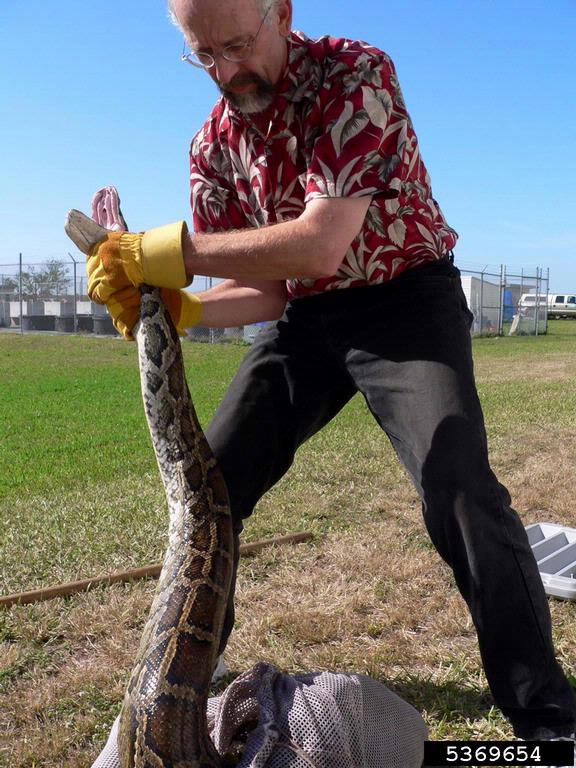
\includegraphics[width=0.4\textwidth]{start.jpg}
    \end{center}
\end{frame}

\begin{frame}[fragile]
    \frametitle{IPython}
    \begin{itemize}
        \item Enhanced interactive Python shell
        \item Main features
        \begin{itemize}
            \item Dynamic introspection and help
            \item Searching through modules and namespaces
            \item Tab completion
            \item Complete system shell access
            \item Session logging \& restoring
            \item Verbose and colored exception traceback printouts
            \item Highly configurable, programmable (Macros, Aliases)
            \item Embeddable
        \end{itemize}
    \end{itemize}
\end{frame}

\begin{frame}[fragile]
    \frametitle{IPython: Getting Help}
    \begin{itemize}
    \item Get help for a function:
    \begin{myColorBox}{0.9}{} \verb#>>> command?#\end{myColorBox}
    \item Have a look at the implementation:
    \begin{myColorBox}{0.9}{} \verb#>>> command??#\end{myColorBox}
    \item Search for variables/functions/modules starting with 'ab':
    \begin{myColorBox}{0.9}{} \verb#>>> ab<Tab>#\end{myColorBox}
    \item Which objects are assigned anyway? 
    \begin{myColorBox}{0.9}{} \verb#>>> whos#\end{myColorBox}
    \item What attributes/methods are there? 
    \begin{myColorBox}{0.9}{}\verb#>>> object.<Tab>#\end{myColorBox}
    \item Get help for a object/class method/attribute:
    \begin{myColorBox}{0.9}{} \verb#>>> object.command?#\end{myColorBox}
    \end{itemize}
\end{frame}

\begin{frame}[fragile]
    \frametitle{Python Data Types - Primitives}
    \begin{center}
      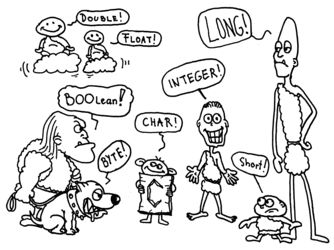
\includegraphics[width=0.6\textwidth]{data.jpg}
    \end{center}
\end{frame}


\begin{frame}[fragile]
    \frametitle{Python Data Types: Numbers}
    \begin{myColorBox}{0.9}{}
\begin{verbatim}
>>> a = 17
>>> type(a)
<type 'int'>
\end{verbatim}
    \end{myColorBox}
    \pause
    \begin{myColorBox}{0.9}{}
\begin{verbatim}
>>> a / 10
1
>>> a % 10
7
>>> a / 10.0
1.7
\end{verbatim}
    \end{myColorBox}
    \pause
    \begin{myColorBox}{0.9}{}
\begin{verbatim}
>>> _
1.7
>>> type(_)
<type 'float'>
\end{verbatim}
    \end{myColorBox}
\end{frame}


\begin{frame}[fragile]
    \frametitle{Python Data Types: Numbers}
    \begin{myColorBox}{0.91}{}
\begin{verbatim}
>>> x = y = z = 0
\end{verbatim}
    \end{myColorBox}
    \pause
    \begin{myColorBox}{0.91}{}
\begin{verbatim}
>>> a=3.0+4.0j
>>> float(a)
Traceback (most recent call last):
\dots
TypeError: can't convert complex to float
>>> a.real
3.0
>>> a.imag
4.0
>>> abs(a)  # sqrt(a.real**2 + a.imag**2)
5.0
\end{verbatim}
    \end{myColorBox}
\end{frame}


\begin{frame}[fragile]
    \frametitle{Python Data Types: Numbers}
    \begin{myColorBox}{0.9}{}
\begin{verbatim}
>>> a = 17
>>> a = a + 1
>>> a
18
\end{verbatim}
    \end{myColorBox}
    \pause
    \begin{myColorBox}{0.9}{}
\begin{verbatim}
>>> a+=2
>>> a
20
\end{verbatim}
    \end{myColorBox}
    \pause
    \begin{myColorBox}{0.9}{}
\begin{verbatim}
>>> a++
     a++
        ^
SyntaxError: invalid syntax
\end{verbatim}
    \end{myColorBox}
\end{frame}

\begin{frame}[fragile]
    \frametitle{Python Data Types: Strings}
    \begin{myColorBox}{0.9}{}
\begin{verbatim}
>>> 'spam eggs'
'spam eggs'
>>> "doesn't"
"doesn't"
\end{verbatim}
    \end{myColorBox}
    \pause
    \begin{myColorBox}{0.9}{}
\begin{verbatim}
>>> 'doesn\'t'
"doesn't"
>>> '"Yes," he said.'
'"Yes," he said.'
>>> "\"Yes,\" he said."
'"Yes," he said.'
>>> '"Isn\'t," she said.'
'"Isn\'t," she said.'
\end{verbatim}
    \end{myColorBox}
\end{frame}


\begin{frame}[fragile]
    \frametitle{Python Data Types: Strings}
    \begin{myColorBox}{0.9}{}
\begin{verbatim}
>>> hello = "This is a rather long string\n\
... containing several lines of text.\n\
...     Note that whitespace at the beginning of \
...  the line is significant."
\end{verbatim}
    \end{myColorBox}
    \pause
    \begin{myColorBox}{0.9}{}
\begin{verbatim}
>>> print """
... Usage: thingy [OPTIONS]
...      -h                Display this message
...      -H hostname       Hostname to connect to
... """
\end{verbatim}
    \end{myColorBox}
\end{frame}


\begin{frame}[fragile]
    \frametitle{Python Data Types: Strings}
    \begin{myColorBox}{0.9}{}
\begin{verbatim}
>>> ’sp’ + ’am’
’spam’
>>> ’spam’ * 10
’spamspamspamspamspamspamspamspamspamspam’
\end{verbatim}
    \end{myColorBox}
    \pause
    \begin{myColorBox}{0.9}{}
\begin{verbatim}
>>> a = "Munich Earth Skience School"
>>> a[0]
'M'
>>> a[0:1]
'M' # different than in other languages!
>>> a[1:4]
'uni'
>>> a[-6:]
'School'
\end{verbatim}
    \end{myColorBox}
\end{frame}


\begin{frame}[fragile]
    \frametitle{Python Data Types: Strings}
    \begin{myColorBox}{0.9}{}
\begin{verbatim}
>>> a = 'spam'
>>> a[3] = 'n' # strings are immutable
Traceback (most recent call last):
...
TypeError: 'str' object does not support item assignment
\end{verbatim}
    \end{myColorBox}
    \pause
    \begin{myColorBox}{0.9}{}
\begin{verbatim}
>>> b = a[:-1] + 'n'
>>> b
'span'
\end{verbatim}
    \end{myColorBox}
    \pause
    \begin{myColorBox}{0.9}{}
\begin{verbatim}
>>> len(b)
4
\end{verbatim}
    \end{myColorBox}
\end{frame}


\begin{frame}[fragile]
    \frametitle{Python Data Types: Strings}
    Strings are objects with many useful methods:
    \begin{myColorBox}{0.9}{}
\begin{verbatim}
>>> a = "Munich Earth Skience School"
>>> a.find('Earth')
7
\end{verbatim}
    \end{myColorBox}
    \pause
    \begin{myColorBox}{0.9}{}
\begin{verbatim}
>>> a.split()
['Munich', 'Earth', 'Skience', 'School']
\end{verbatim}
    \end{myColorBox}
    \pause
    \begin{myColorBox}{0.9}{}
\begin{verbatim}
>>> ' * '.join(_)
'Munich * Earth * Skience * School'
\end{verbatim}
    \end{myColorBox}
    There are more useful \verb#string# methods like \verb#startswith#, \verb#endswith#, \verb#lower#, \verb#upper#,
    \verb#ljust#, \verb#rjust#, \verb#center#, \verb#...#. See Python Library Reference.
\end{frame}

\begin{frame}[fragile]
    \frametitle{Python Data Types - Container}
    \begin{center}
      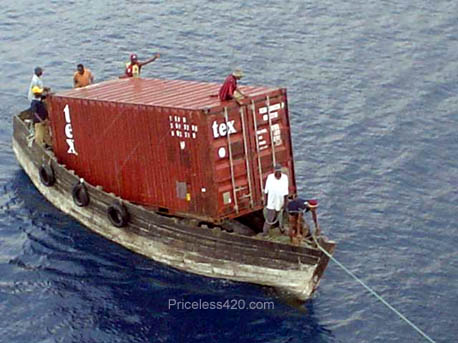
\includegraphics[width=0.6\textwidth]{container.jpg}
    \end{center}
\end{frame}


\begin{frame}[fragile]
    \frametitle{Python Data Types: Lists}
    \begin{myColorBox}{0.9}{}
\begin{verbatim}
>>> a = ['spam', 'eggs', 100, 1234]
>>> a
['spam', 'eggs', 100, 1234]
\end{verbatim}
    \end{myColorBox}
    \pause
    \begin{myColorBox}{0.9}{}
\begin{verbatim}
>>> a[0]
'spam'
>>> a[3]
1234
>>> a[-2]
100
>>> a[:2] + ['bacon', 2*2]
['spam', 'eggs', 'bacon', 4]
>>> 2*a[:3] + ['Boo!']
['spam', 'eggs', 100, 'spam', 'eggs', 100, 'Boo!']
\end{verbatim}
    \end{myColorBox}
\end{frame}

\begin{frame}[fragile]
    \frametitle{Python Data Types: Lists}
    \begin{myColorBox}{0.9}{}
\begin{verbatim}
>>> a
['spam', 'eggs', 100, 1234]
>>> a[2] = a[2] + 23 # lists are mutable
>>> a
['spam', 'eggs', 123, 1234]
\end{verbatim}
    \end{myColorBox}
    \pause
    \begin{myColorBox}{0.9}{}
\begin{verbatim}
>>> a[0:2] = [1, 12] # Replace some items
>>> a
[1, 12, 123, 1234]
>>> a[0:2] = [] # Remove some
>>> a
[123, 1234]
>>> a[1:1] = ['bletch', 'xyzzy'] # Insert some
>>> a
[123, 'bletch', 'xyzzy', 1234]
\end{verbatim}
    \end{myColorBox}
\end{frame}


\begin{frame}[fragile]
    \frametitle{Python Data Types: Lists}
    \begin{myColorBox}{0.9}{}
\begin{verbatim}
>>> a[::-1]
[1234, 'xyzzy', 'bletch', 123]
\end{verbatim}
    \end{myColorBox}
    \pause
    \begin{myColorBox}{0.9}{}
\begin{verbatim}
>>> len(a)
4
\end{verbatim}
    \end{myColorBox}
    \pause
    \begin{myColorBox}{0.9}{}
\begin{verbatim}
>>> a[:] = [] # Clear the list
>>> a
[]
\end{verbatim}
    \end{myColorBox}
    \pause
    There are more useful \verb#list# methods like \verb#append#, \verb#insert#, \verb#remove#, \verb#sort#,
    \verb#pop#, \verb#index#, \verb#reverse#, \verb#...#. See Python Library Reference.
\end{frame}


\begin{frame}[fragile]
    \frametitle{Python Data Types: Tuples, Boolean \& None}
    Tuples
    \begin{itemize}
        \item Immutable lists created by \textbf{round} parantheses
        \item Parantheses can be ommited in many cases.
    \end{itemize}
    \begin{myColorBox}{0.9}{}
\begin{verbatim}
>>> t = (12345, 54321, 'hello!')
>>> t[0]
12345
\end{verbatim}
    \end{myColorBox}
\pause
Boolean
        \begin{myColorBox}{0.9}{}
\begin{verbatim}
>>> type(True)
<type 'bool'>
\end{verbatim}
    \end{myColorBox}
\pause
None
        \begin{myColorBox}{0.9}{}
\begin{verbatim}
>>> a = None
>>> type(a)
<type 'NoneType'>
\end{verbatim}
    \end{myColorBox}
\pause

\end{frame}

\begin{frame}[fragile]
    \frametitle{Python Data Types: Dictionaries}
    \begin{myColorBox}{0.9}{}
\begin{verbatim}
>>> tel = {'jack': 4098, 'sape': 4139}
>>> tel['guido'] = 4127
>>> tel
{'sape': 4139, 'guido': 4127, 'jack': 4098}
>>> tel['jack']
4098
>>> del tel['sape']
>>> tel['irv'] = 4127
>>> tel
{'guido': 4127, 'irv': 4127, 'jack': 4098}
>>> tel.keys()
['guido', 'irv', 'jack']
>>> 'guido' in tel
True
\end{verbatim}
    \end{myColorBox}
\end{frame}


\begin{frame}[fragile]
    \frametitle{Python Data Types: NumPy Arrays}
We need to import \verb#numpy# for the following examples:
    \begin{myColorBox}{0.9}{}
\begin{verbatim}
from numpy import *
\end{verbatim}
    \end{myColorBox}
    \begin{myColorBox}{0.9}{}
\begin{verbatim}
>>> a = array( [2, 3, 4] )
>>> a
array([2, 3, 4])
>>> type(a) 
<type 'numpy.ndarray'>
\end{verbatim}
    \end{myColorBox}
    \pause
    \begin{myColorBox}{0.9}{}
\begin{verbatim}
>>> b =array( [ (1.5, 2, 3), (4, 5, 6) ] )
>>> b
array([[ 1.5,  2. ,  3. ],
       [ 4. ,  5. ,  6. ]])
\end{verbatim}
    \end{myColorBox}
\end{frame}

\begin{frame}[fragile]
    \frametitle{Python Data Types: NumPy Arrays}
    \begin{myColorBox}{0.9}{}
\begin{verbatim}
>>> b.ndim     # number of dimensions
2
>>> b.shape    # the dimensions
(2, 3)
>>> b.dtype    # the type (8 byte floats)
dtype('float64')
>>> b.itemsize # the size of the type
8
\end{verbatim}
    \end{myColorBox}
    \pause    
    \begin{myColorBox}{0.9}{}
\begin{verbatim}
>>> c = array( [ [1, 2], [3, 4] ], dtype=complex )
>>> c
array([[ 1.+0.j,  2.+0.j],
       [ 3.+0.j,  4.+0.j]])
\end{verbatim}
    \end{myColorBox}
\end{frame}

\begin{frame}[fragile]
    \frametitle{Python Data Types: NumPy Arrays}
    \begin{myColorBox}{0.9}{}
\begin{verbatim}
>>> zeros( (3, 4) )  # parameter specify the shape
array([[0.,  0.,  0.,  0.],
       [0.,  0.,  0.,  0.],
       [0.,  0.,  0.,  0.]])
>>> ones( (2, 3, 4), dtype=int16 ) # dtype specified
array([[[ 1, 1, 1, 1],
        [ 1, 1, 1, 1],
        [ 1, 1, 1, 1]],
       [[ 1, 1, 1, 1],
        [ 1, 1, 1, 1],
        [ 1, 1, 1, 1]]], dtype=int16)
\end{verbatim}
    \end{myColorBox}
Supported data types: bool, uint8, uint16, uint32, uint64, int8, int16, int32, int64, float32, float64, float96, complex64, complex128, complex192 
\end{frame}

\begin{frame}[fragile]
    \frametitle{Python Data Types: NumPy Arrays}
    \begin{myColorBox}{0.9}{}
\begin{verbatim}
>>> empty( (2,3) )
array([[  3.73603959e-262,   ...,   ...],
       [  5.30498948e-313,   ...,   ...]])
\end{verbatim}
    \end{myColorBox}
    \pause
    \begin{myColorBox}{0.9}{}
\begin{verbatim}
>>> arange( 10, 30, 5 )
array([10, 15, 20, 25])
>>> arange( 0, 2, 0.3 ) # it accepts float arguments
array([ 0. ,  0.3,  0.6,  0.9,  1.2,  1.5,  1.8])
\end{verbatim}
    \end{myColorBox}
    \pause
    \begin{myColorBox}{0.9}{}
\begin{verbatim}
>>> linspace( 0, 2, 9 ) # 9 numbers from 0 to 2
array([ 0.  ,  0.25,  0.5 ,  0.75, ...,  2.  ])
>>> x = linspace( 0, 2*pi, 100 )
>>> f = sin(x)
\end{verbatim}
    \end{myColorBox}
\end{frame}

\begin{frame}[fragile]
    \frametitle{Python Data Types: NumPy Arrays}
    \begin{myColorBox}{0.9}{}
\begin{verbatim}
>>> A = array( [[1,1], [0,1]] )
>>> B = array( [[2,0], [3,4]] )
>>> A*B  # elementwise product
array([[2, 0], 
       [0, 4]])
>>> dot(A,B) # matrix product
array([[5, 4],
       [3, 4]])
>>> mat(A)*mat(B) # matrix product
matrix([[5, 4],
       [3, 4]])
\end{verbatim}
    \end{myColorBox}
There are further functions for array creation, conversions, manipulation, querying, ordering, operations, statistics, basic linear algebra. See NumPy documentation.
\end{frame}


\begin{frame}[fragile]
    \frametitle{Flow Control}
    \begin{center}
      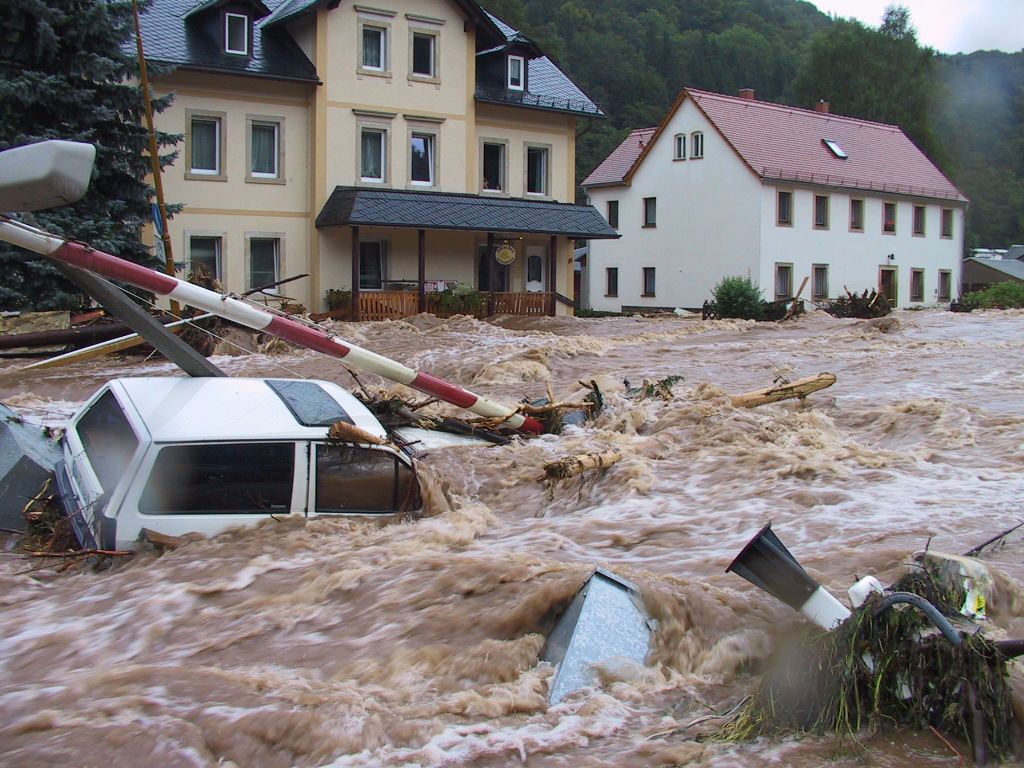
\includegraphics[width=0.7\textwidth]{flowcontrol.jpg}
    \end{center}
\end{frame}


\begin{frame}[fragile]
    \frametitle{Flow Control: if-statement}
    \begin{myColorBox}{0.9}{}
\begin{verbatim}
>>> x = int(raw_input("Please enter an integer: "))
Please enter an integer: 42
>>> if x < 0:
...      print 'Negative'
... elif x == 0:
...      print 'Zero'
... elif x == 1:
...      print 'Single'
... else:
...      print 'More'
...
More
\end{verbatim}
    \end{myColorBox}
\end{frame}


\begin{frame}[fragile]
    \frametitle{Flow Control: for-statement}
    \begin{myColorBox}{0.9}{}
\begin{verbatim}
>>> a = ['cat', 'window', 'defenestrate']
>>> for x in a:
...     print x, len(x)
...
cat 3
window 6
defenestrate 12
\end{verbatim}
    \end{myColorBox}
    \pause
    \begin{myColorBox}{0.9}{}
\begin{verbatim}
>>> for i in range(0, 6, 2):
...     print i
...
0
2
4
\end{verbatim}
    \end{myColorBox}
\end{frame}


\begin{frame}[fragile]
    \frametitle{Flow Control: while-statement}
    \begin{myColorBox}{0.9}{}
\begin{verbatim}
>>> import time
>>> i = 1
>>> while True:
...     i = i * 1000 # same as: i *= 1000
...     print repr(i)
...     time.sleep(1) # wait one second
...
1000
1000000
1000000000
1000000000000L # <- type conversion occured!
1000000000000000L
# ... continues until memory is exhausted!
\end{verbatim}
    \end{myColorBox}
\end{frame}


\begin{frame}[fragile]
    \frametitle{Flow Control: continue \& break}
The \verb#break# statement breaks out of the smallest enclosing for or while loop.
    \begin{myColorBox}{0.9}{}
\begin{verbatim}
>>> for i in range(0, 100000):
...     if i>50:
...         print i
...         break
...
51
\end{verbatim}
    \end{myColorBox}
\pause
The \verb#continue# statement continues with the next iteration of the loop.
    \begin{myColorBox}{0.9}{}
\begin{verbatim}
>>> for i in range(0, 100000):
...     if i!=50:
...         continue
...     print i
...
50
\end{verbatim}
    \end{myColorBox}
\end{frame}


\begin{frame}[fragile]
    \frametitle{Functions}
Defining a function which returns a Fibonacci series up to n.
    \begin{myColorBox}{0.9}{}
\begin{verbatim}
>>> def fib2(n):
...     """Return the Fibonacci series up to n."""
...     result = []
...     a, b = 0, 1
...     while a < n:
...         result.append(a)
...         a, b = b, a+b
...     return result
\end{verbatim}
    \end{myColorBox}
\pause
Now call the function we just defined:
    \begin{myColorBox}{0.9}{}
\begin{verbatim}
>>> fib(100)
[0, 1, 1, 2, 3, 5, 8, 13, 21, 34, 55, 89]
\end{verbatim}
    \end{myColorBox}
\end{frame}

\begin{frame}[fragile]
    \frametitle{Functions}
    \begin{myColorBox}{0.9}{}
\begin{verbatim}
def birthday2(name, age = 1):
    msg = "Happy birthday, %s! You're %d today."
    print  msg % (name, age)
\end{verbatim}
    \end{myColorBox}
\pause
    \begin{myColorBox}{0.9}{}
\begin{verbatim}
>>> birthday2("Katherine")
Happy birthday, Katherine! You're 1 today.
\end{verbatim}
    \end{myColorBox}
\pause
    \begin{myColorBox}{0.9}{}
\begin{verbatim}
>>> birthday2(age = 12, name = "Katherine")
Happy birthday, Katherine! You're 12 today.
\end{verbatim}
    \end{myColorBox}
\pause
    \begin{myColorBox}{0.9}{}
\begin{verbatim}
>>> birthday2("Katherine", 14)
Happy birthday, Katherine! You're 14 today.
\end{verbatim}
    \end{myColorBox}
\end{frame}

\begin{frame}[fragile]
    \frametitle{Input \& Output}
    \begin{center}
      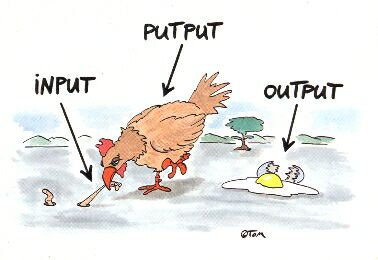
\includegraphics[width=0.6\textwidth]{io.jpg}
    \end{center}
\end{frame}

\begin{frame}[fragile]
    \frametitle{File Handling}
    Use \verb#open(filename, mode)# to open a file. Returns a File Object.
    \begin{myColorBox}{0.9}{}
\begin{verbatim}
fh = open('/path/to/file', 'r')
\end{verbatim}
    \end{myColorBox}
   \begin{itemize}
   \item Some possible modes:
   \begin{itemize}
        \item r: Open text file for read.
        \item w: Open text file for write.
        \item a: Open text file for append.
        \item rb: Open binary file for read.
        \item wb: Open binary file for write.
    \end{itemize}
    \end{itemize}
    Use \verb#close()# to close a given File Object.
    \begin{myColorBox}{0.9}{}
\begin{verbatim}
fh.close()
\end{verbatim}
    \end{myColorBox}
\end{frame}

\begin{frame}[fragile]
    \frametitle{Reading Files}
Read a quantity of data from a file:
    \begin{myColorBox}{0.9}{}
\begin{verbatim}
s = fh.read( size ) # size: number of bytes to read
\end{verbatim}
    \end{myColorBox}
\pause
Read entire file
    \begin{myColorBox}{0.9}{}
\begin{verbatim}
s = fh.read()
\end{verbatim}
    \end{myColorBox}
\pause
Read one line from file:
    \begin{myColorBox}{0.9}{}
\begin{verbatim}
s = fh.readline()
\end{verbatim}
    \end{myColorBox}
\pause
Get all lines of data from the file into a list:
    \begin{myColorBox}{0.9}{}
\begin{verbatim}
list = fh.readlines()
\end{verbatim}
    \end{myColorBox}
\pause
Iterate over each line in the file:
    \begin{myColorBox}{0.9}{}
\begin{verbatim}
for line in fh:
    print line,
\end{verbatim}
    \end{myColorBox}
\end{frame}

\begin{frame}[fragile]
    \frametitle{Writing Files}
Write a string to the file:
    \begin{myColorBox}{0.9}{}
\begin{verbatim}
fh.write( string )
\end{verbatim}
    \end{myColorBox}
\pause
Write several strings to the file:
    \begin{myColorBox}{0.9}{}
\begin{verbatim}
fh.writelines( sequence )
\end{verbatim}
    \end{myColorBox}
\end{frame}

\begin{frame}[fragile]
    \frametitle{Errors and Exceptions}
    \begin{center}
      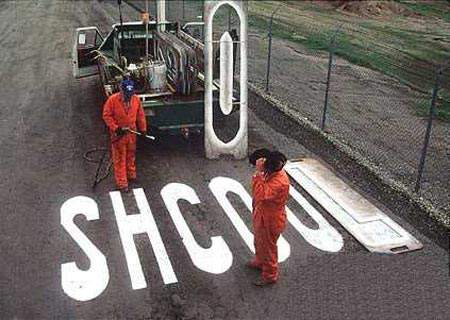
\includegraphics[width=0.7\textwidth]{shcool.jpg}
    \end{center}
\end{frame}

\begin{frame}[fragile]
    \frametitle{Exceptions}
    \begin{myColorBox}{0.9}{}
\small
\begin{verbatim}
>>> 10 * (1/0)
Traceback (most recent call last):
  File "<stdin>", line 1, in ?
ZeroDivisionError: integer division or modulo by zero
\end{verbatim}
    \end{myColorBox}
    \pause    
    \begin{myColorBox}{0.9}{}
\small
\begin{verbatim}
>>> 4 + muh*3
Traceback (most recent call last):
  File "<stdin>", line 1, in ?
NameError: name 'muh' is not defined
\end{verbatim}
    \end{myColorBox}
    \pause    
    \begin{myColorBox}{0.9}{}
\small
\begin{verbatim}
>>> '2' + 2
Traceback (most recent call last):
  File "<stdin>", line 1, in ?
TypeError: cannot concatenate 'str' and 'int' objects
\end{verbatim}
    \end{myColorBox}
\end{frame}


\begin{frame}[fragile]
    \frametitle{Handling Exceptions}
    \begin{myColorBox}{0.9}{}
\small
\begin{verbatim}
def divide(x, y):
    try:
        result = x / y
    except ZeroDivisionError:
        print "division by zero!"
    except TypeError:
        print "unsupported type!"
    else:
        print "result is", result
\end{verbatim}
    \end{myColorBox}
    \begin{myColorBox}{0.9}{}
\small
\begin{verbatim}
>>> divide(2, 1)
result is 2
>>> divide(2, 0)
division by zero!
>>> divide(2, 'bbb')
unsupported type!
\end{verbatim}
    \end{myColorBox}
\end{frame}


%\section{Overview}
%\subsection{Overview}
%\begin{frame}[fragile]
%    \frametitle{ObsPy Data Types -- Why bother?}
%    %Why bother to define object classes??\\
%    \begin{itemize}
%    \item ... we want to unify data from different sources in a common structure.
%    \begin{verbatim}
%    st = read("file.mseed")
%    st += read("file.sac")
%    st += client_arclink.getWaveform(...)
%    st += client_iris.getWaveform(...)
%    \end{verbatim}
%    \end{itemize}
%\end{frame}

%\begin{frame}[fragile]
%    \frametitle{ObsPy Data Types -- Why bother?}
%    %Why bother to define object classes??\\
%    \begin{itemize}
%    \item ... they know how to behave by themselves if we tell them once.
%    \begin{verbatim}
%    utcdatetime + 10
%    st += st2
%    st.filter("lowpass", freq=1)
%    \end{verbatim}
%    \end{itemize}
%\end{frame}

%\begin{frame}[fragile]
%    \frametitle{ObsPy Data Types -- Why bother?}
%    %Why bother to define object classes??\\
%    \begin{itemize}
%    \item ... there is less room for user errors.
%    \begin{verbatim}
%    #st = client.getWaveform(..., channel="BHZ")
%    st = client.getWaveform(..., channel="HHZ")
%    data = st[0].data
%
%    data = obspy.signal.lowpass(data, freq=1, df=20)
%    \end{verbatim}
%    \end{itemize}
%\end{frame}

%\begin{frame}[fragile]
%    \frametitle{ObsPy Data Types -- Why bother?}
%    %Why bother to define object classes??\\
%    \begin{itemize}
%    \item ... the code gets much shorter and better readable.\\
%    \vspace*{1.0em}
%    How about...
%    \begin{verbatim}
%    st = read("file")
%    from obspy.signal import lowpass
%    num_traces = len(st)
%    for i in range(num_traces):
%        df = st[i].stats.sampling_rate
%        st[i].data = lowpass(st[i].data, freq=1, df=df)
%    \end{verbatim}
%    ...against:
%    \begin{verbatim}
%    st = read("file")
%    st.filter("lowpass", freq=1)
%    \end{verbatim}
%    \end{itemize}
%\end{frame}

\begin{frame}[fragile]
    \frametitle{ObsPy}
    \begin{center}
      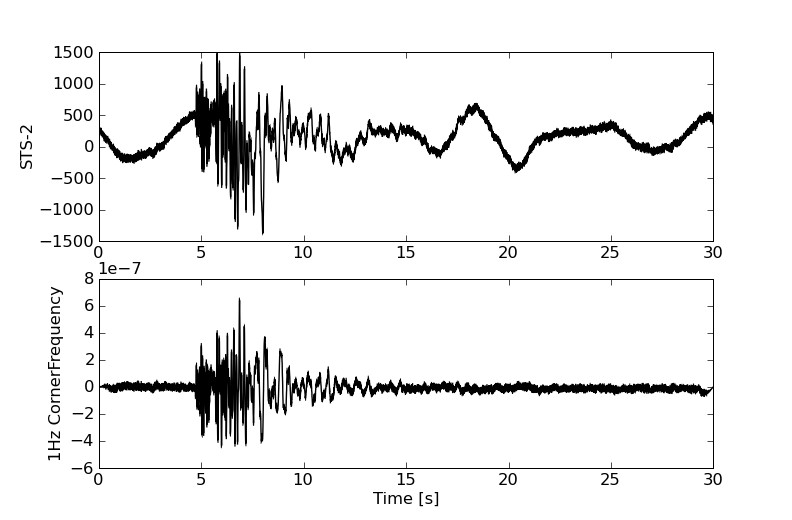
\includegraphics[width=0.7\textwidth]{arclink.png}
    \end{center}
\end{frame}

\begin{frame}[fragile]
    \frametitle{ObsPy}
    \begin{itemize}
        \item Python toolbox for seismologists
        \item Modular architecture
        \item Waveform data: GSE2, MiniSEED, SAC, WAV, Q/ASCII
        \item Inventory data: Dataless SEED, XML-SEED, RESP
        \item Data request clients: ArcLink/WebDC, IRIS DHI/Fissures/WS, SeisHub, NERIES WS
        \item Various pickers, filters and plot routines
        \item Waveform indexer
    \end{itemize}
\end{frame}

\begin{frame}[fragile]
    \frametitle{ObsPy}
    \begin{itemize}
        \item Open source (LGPL or GPL)
        \item 6 core developers
        \item Test-driven development (TDD), currently more than 470 unit tests (http://tests.obspy.org)
        \item Reliance of well-known third-party libraries (numpy, scipy, matplotlib)
        \item Reusing well established code, e.g. libmseed, GSE UTI
        \item Automatic generated API documentation
        \item Binary distributions: Python Package Index (PyPI), Windows Installer (\& Debian packages)
        \item Central source code repository, community webpage, tutorials, installation instructions, ticket system, mailing list:
    \end{itemize}
    \begin{center}
    \textbf{http://www.obspy.org}
    \end{center}
\end{frame}

\begin{frame}[fragile]
    \frametitle{Need a break..?}
    \begin{center}
      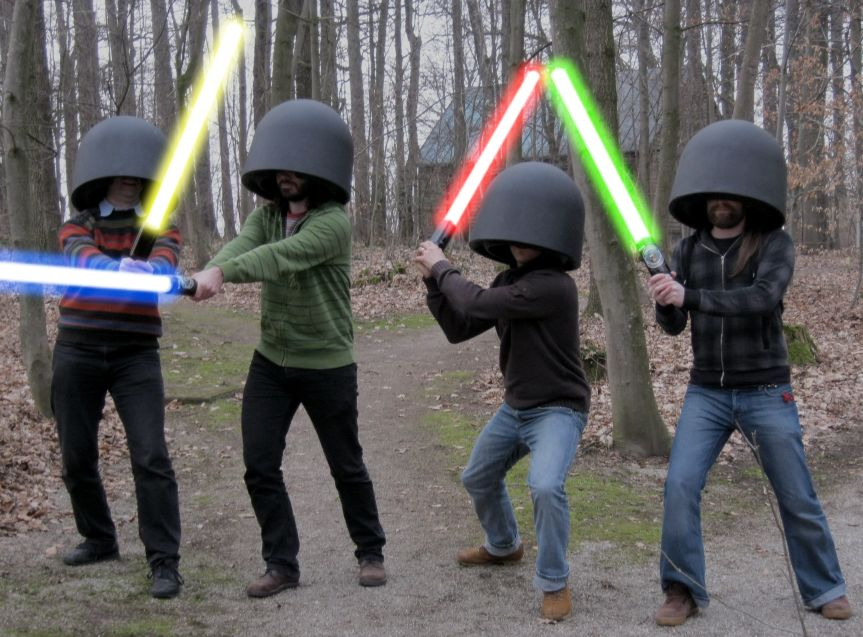
\includegraphics[width=0.7\textwidth]{obstroopers.jpg}
    \end{center}
\end{frame}

\begin{frame}[fragile]
    \frametitle{How to Work on the Practicals..}
    \begin{itemize}
    \item Either..
        \begin{itemize}
        \item work line by line in IPython shell
        \item when it's working: save history and condense it
    \begin{verbatim}
    >>> %history [number_of_lines] [-n] [-f output_file]
    \end{verbatim}
        \end{itemize}
    \item or..
        \begin{itemize}
        \item work on your program in a text editor
        \item in a second window, run program in an IPython shell and continue work at the end
    \begin{verbatim}
    $ ipython -i
    >>> run -i PROGRAM.PY
    \end{verbatim}
            \begin{itemize}
            \item (caution: best do this in a 'fresh' IPython shell)
            \end{itemize}
        \item extend program with appropriate lines of code and run it again in a new IPython shell
        \end{itemize}
    \end{itemize}
\end{frame}

\begin{frame}[fragile]
    \frametitle{Getting Help..}
    IPython
    \begin{itemize}
    \item get help for a function: \verb#>>> command?#
    \item have a look at the implementation: \verb#>>> command??#
    \item search for variables/functions/modules starting with 'ab': \verb#>>> ab<Tab>#
    \item what's the value? \verb#>>> variable#
    \item what's the type? \verb#>>> type(variable)#
    \item which variables are assigned anyway?? \verb#>>> whos#
    \item what attributes/methods are there? \verb#>>> variable.<Tab>#
    \item get help for a variable's method: \verb#>>> variable.command?#
    \item what functions are available in a module? \verb#>>> module.<Tab>#
    \end{itemize}
\end{frame}

\begin{frame}[fragile]
    \frametitle{Getting Help..}
    \begin{itemize}
    \item ObsPy web pages
        \begin{itemize}
        \item Tutorial
            \begin{itemize}
            \item \url{http://obspy.org/wiki/ObspyTutorial}
            \item \url{file:///home/messuser/obspy/tutorial/ObspyTutorial.html}
            \end{itemize}
        \item API
            \begin{itemize}
            \item \url{http://docs.obspy.org/}
            \item \url{file:///home/messuser/obspy/docs/index.html}
            \end{itemize}
        \end{itemize}
    \item Python/Numpy/Scipy API
        \begin{itemize}
        \item \url{http://docs.python.org/}
        \item \url{file:///home/messuser/obspy/python/python-docs/index.html}
        \item \url{http://docs.scipy.org/doc/numpy/reference/}
        \item \url{file:///home/messuser/obspy/python/numpy-docs/index.html}
        \item \url{http://docs.scipy.org/doc/scipy/reference/}
        \item \url{file:///home/messuser/obspy/python/scipy-docs/index.html}
        \end{itemize}
    \end{itemize}
\end{frame}

\begin{frame}[fragile]
    \frametitle{ObsPy Data Types -- Overview}
    \begin{itemize}
    \item \verb#UTCDateTime#
        \begin{itemize}
        \item extension of the Python \verb#datetime# object
        \item stores a time stamp
        \end{itemize}
    \item \verb#Stats#
        \begin{itemize}
        \item extension of the Python \verb#dict# object
        \item stores header information of waveforms
        \end{itemize}
    \item \verb#Trace#
        \begin{itemize}
        \item stores a single-channel, continuous piece of waveform data
        \item consisting of waveform data and header information
        \end{itemize}
    \item \verb#Stream#
        \begin{itemize}
        \item stores multiple traces (e.g. Z, N, E traces of one station)
        \end{itemize}
    \item all of them defined in \verb#obspy.core#
        \begin{itemize}
        \item \verb#from obspy.core import UTCDateTime#
        \end{itemize}
    \end{itemize}
\end{frame}

\begin{frame}[fragile]
    \frametitle{ObsPy Data Types -- \tt{UTCDateTime}}
    \begin{itemize}
    \item \verb#UTCDateTime#
        \begin{itemize}
        \item used to handle all time information in ObsPy
        \item initialize via
            \begin{itemize}
            \item \verb#t = UTCDateTime("2011-02-21T08:00:00.00Z")#
            \item \verb#t = UTCDateTime(2011, 2, 21, 8)#
            \item ...
            \end{itemize}
        \item several attributes/methods\\ (e.g. \verb#t.microsecond#, \verb#t.julday#, \verb#t.weekday()#, ...)
        \item important operations
            \begin{itemize}
            \item subtracting two \verb#UTCDateTime# objects gives time difference in seconds
            \item adding/subtracting \verb#int#/\verb#float# returns new \verb#UTCDateTime# object
            \end{itemize}
        \item see \href{file:///home/messuser/obspy/docs/packages/auto/obspy.core.utcdatetime.UTCDateTime.html}{ObsPy documentation}
        \end{itemize}
    \end{itemize}
\end{frame}

\begin{frame}[fragile]
    \frametitle{Exercises -- \tt{UTCDateTime}}
    \begin{itemize}
    \item A
        \begin{itemize}
        \item the morning sessions start at 8 and are 3 hours..\\ assume we
              want to have the coffee break 1234 seconds and 5 microseconds before
              the session ends. What time is the break?
        \item assume you had your last cup of coffee yesterday at breakfast. How many
              minutes do you have to survive with that cup of coffee?
        \end{itemize}
    \end{itemize}
    \begin{itemize}
    \item<2> B
        \begin{itemize}
        \item<2> how many days from today is your birthday this year?
        \item<2> what day of week is it?
        \item<2> you want to have your birthday party at the first saturday after your
              birthday, what date is the party?
        \end{itemize}
    \end{itemize}
    \begin{itemize}
    \item<2> C
        \begin{itemize}
        \item<2> some of your friends always seem to find an excuse not to come..\\
              for the next fifty years print the date of your party sticking to
              that scheme
        \item<2> we are superstitious and do not leave the house on friday 13th..\\
              print a list of dates and count the days we have to take off from
              now till the end of next year..
        \end{itemize}
    \end{itemize}
\end{frame}

\begin{frame}[fragile]
    \frametitle{ObsPy Data Types -- \tt{Stats}}
    \begin{itemize}
    \item \verb#Stats# -- header information for waveform data
        \begin{itemize}
        \item contains at least the following keys
            \begin{itemize}
            \item \verb#stats.network# -- network code (\verb#str#)
            \item \verb#stats.station# -- station code (\verb#str#)
            \item \verb#stats.location# -- location code (\verb#str#)
            \item \verb#stats.channel# -- channel code (\verb#str#)
            \item \verb#stats.starttime# -- time of first sample (\verb#UTCDateTime#)
            \item \verb#stats.sampling_rate# -- sampling rate in \verb#Hz# (\verb#float#)
            \item \verb#stats.npts# -- number of samples (\verb#int#)
            \end{itemize}
        \item derived keys
            \begin{itemize}
            \item \verb#stats.endtime# -- time of last sample (\verb#UTCDateTime#)
            \item \verb#stats.delta# -- sampling interval (\verb#float#)
            \end{itemize}
        \item optional keys
            \begin{itemize}
            \item \verb#stats._format# -- format of original data file (\verb#str#, e.g. \verb#"MSEED"#)
            \item \verb#stats.paz# -- poles, zeros, sensitivity and gain of instrument (\verb#dict#)
            \item \verb#stats.coordinates# -- longitude, latitude and elevation of station (\verb#dict#)
            \item ...
            \end{itemize}
        \item see \href{file:///home/messuser/obspy/docs/packages/auto/obspy.core.trace.Stats.html}{ObsPy documentation}
        \end{itemize}
    \end{itemize}
\end{frame}

\begin{frame}[fragile]
    \frametitle{ObsPy Data Types -- \tt{Trace}}
    \begin{itemize}
    \item \verb#Trace# -- continuous waveform data
        \begin{itemize}
        \item usually constructed internally during \verb#read(...)# or \verb#getWaveform(...)#
        \item consists of
            \begin{itemize}
            \item \verb#tr.data# -- waveform data as a \verb#numpy.ndarray# instance
            \item \verb#tr.stats# -- header information as a \verb#Stats# instance
            \end{itemize}
        \item built-in methods
            \begin{itemize}
            \item \verb#tr.id# -- complete channel id in SEED standard (e.g. \verb#"BW.RJOB..BHZ"#)
            \item \verb#tr.plot()# -- shows preview plot of trace
            \item \verb#tr.copy()# -- returns copy of trace (most operations work in-place)
            \item \verb#tr.trim(starttime, endtime)# -- cut trace to specified time span
            \item \verb#tr.filter("type", **kwargs)# -- filter waveform data
            \item \verb#tr.simulate(paz_remove, paz_simulate, **kwargs)#\\ -- apply instrument correction/simulation
            \item \verb#tr.write("filename", "format")# -- write waveform to local file
            \item ...
            \end{itemize}
        \item many built-in methods on \verb#tr.data# (\verb#numpy.ndarray#)!
        \item see \href{file:///home/messuser/obspy/docs/packages/auto/obspy.core.trace.Trace.html}{ObsPy documentation}
        \item see \href{file:///home/messuser/obspy/python/numpy-docs/index.html}{Numpy documentation -- ndarray}
        \end{itemize}
    \end{itemize}
\end{frame}

\begin{frame}[fragile]
    \frametitle{Exercises -- \tt{Trace}}
    \begin{itemize}
    \item A
        \begin{itemize}
        \item make a trace with all zeros (e.g. \verb#numpy.zeros(200)#) and an ideal pulse at the center
        \item fill in some station information (\verb#network#, \verb#station#)
        \item print trace summary and display the preview plot of the trace
        \item change the sampling rate to 20Hz
        \item change the \verb#starttime# to the start time of this sessions
        \item print trace summary and display the preview plot of the trace again
        \end{itemize}
    \end{itemize}
\end{frame}

\begin{frame}[fragile]
    \frametitle{Exercises -- \tt{Trace}}
    \begin{itemize}
    \item B
        \vspace*{0.5em}
        \begin{itemize}
        \item use \verb#tr.filter(...)# and apply a lowpass with 1s corner frequency
        \item display the preview plot, there are a few seconds of zeros that we can cut off
        \item use \verb#tr.trim(...)# to remove some of the zeros at start and end
        \end{itemize}
    \end{itemize}
    \begin{itemize}
    \item C
        \vspace*{0.5em}
        \begin{itemize}
        \item scale up the amplitudes of the trace by a factor of 500
        \item make a copy of the original trace
        \item add standard normal gaussian noise to the copied trace (use \verb#numpy.random.randn(..)#)
        \item change the station name of the copied trace
        \item display the preview plot of the new trace
        \end{itemize}
    \end{itemize}
\end{frame}

\begin{frame}[fragile]
    \frametitle{ObsPy Data Types -- \tt{Stream}}
    \begin{itemize}
    \item \verb#Stream# -- collection of \verb#Trace# objects in a \verb#list#-like container
        \begin{itemize}
        \item usually returned by a \verb#read(...)# or \verb#getWaveform(...)# call
        \item \verb#print st# -- prints summary of all traces
        \item \verb#print len(st)# -- prints number of traces in stream
        \item \verb#list#-like operations
            \begin{itemize}
            \item \verb#st[i]# -- return trace at index \verb#i#
            \item \verb#st.append(tr)# -- add a single trace
            \item \verb#st.extend(st)# -- add a list of traces
            \item \verb#st.remove(tr)# -- remove specified trace from stream
            \item \verb#st.pop(i)# -- remove trace at specified index and return it
            \item \verb#st.sort(...)# -- sort traces in stream according to specified criteria
            \end{itemize}
        \item other built-in methods
            \begin{itemize}
            \item \verb#st.select(**kwargs)#\\ -- return new stream with matching traces (e.g. \verb#component="Z"#)
            \item \verb#st.merge(method)# -- merge traces with identical id
            \item \verb#st.printGaps()# -- prints summary of gaps in the stream
            \end{itemize}
        \item many built-in methods of \verb#Trace# (\verb#trim#, \verb#filter#, \verb#simulate#,... )
        \item see \href{file:///home/messuser/obspy/docs/packages/auto/obspy.core.stream.Stream.html}{ObsPy documentation}
        \end{itemize}
    \end{itemize}
\end{frame}

\begin{frame}[fragile]
    \frametitle{Exercises -- \tt{Stream}}
    \begin{itemize}
    \item A
        \begin{itemize}
        \item read the example earthquake data into a stream object (\verb#read()# without arguments)
        \item print the stream summary and display the preview plot
        \item assign the first trace to a new variable and then remove that trace from the original stream
        \item print the summary for the single trace and for the stream
        \end{itemize}
    \end{itemize}
\end{frame}

\begin{frame}[fragile]
    \frametitle{Exercises -- \tt{Stream}}
    \begin{itemize}
    \item B
        \begin{itemize}
        \item read the example earthquake data again
        \item make a dictionary with \verb#paz# information, assign \verb#poles# at
              \verb#[-0.037+0.037j, -0.037-0.037j]#, \verb#zeros# at \verb#[0j, 0j]#,
              the \verb#sensitivity# of \verb#2.517e9# and unity \verb#gain#
        \item remove the instrument response using this \verb#paz# dictionary
        \item print the data maximum and minimum of the first trace (now in m/s)
        \item save the data to a local file in \verb#MSEED# format
        \end{itemize}
    \end{itemize}
    \begin{itemize}
    \item C
        \begin{itemize}
        \item read the example earthquake data again
        \item change the station name for all traces in the stream
        \item read the example earthquake data again and add the traces to the first stream
        \item print the summary for the resulting stream and display the preview plot
        \item \verb#select# the Z traces and assign this stream to another variable
        \item filter the Z components with a highpass at 5Hz
        \item display the preview plot of the Z component stream
        \item display the preview plot of the original stream
        \end{itemize}
    \end{itemize}
\end{frame}

\begin{frame}[fragile]
    \frametitle{Exercises -- \tt{Stream}}
    \begin{itemize}
    \item D
        \begin{itemize}
        \item fetch earthquake data from a local SeisHub database using \verb#obspy.seishub#
        \item (start the database first, doing \verb#$ seishub-start#)
        \item use \verb#station# HROE in \verb#network# BW and fetch 10 minutes of data starting at October 10th 2008 08:05am
        \item print the stream summary and display the preview plot
        \item fetch event information for the same time span
        \item print the origin time, magnitude and location information of the event
        \end{itemize}
    \end{itemize}
    \vspace*{0.5em}
    \begin{itemize}
    \item<2> E
        \begin{itemize}
        \item<2> do it again using..
        \item<2> \verb#obspy.arclink# (WebDC) for the waveform request\\
                 (use an empty string for \verb#location# and \verb#channel# 'EH*')
        \item<2> \verb#obspy.neries# (NERIES/EMSC) for the event request
        \end{itemize}
    \end{itemize}
\end{frame}

%\begin{frame}[fragile]
%    \frametitle{Useful Constructs}
%    \begin{itemize}
%    \item loop over all traces in a stream \verb#for trace in stream: tr.data = tr.data - tr.data.mean()#
%    \end{itemize}
%\end{frame}

\end{document}
